\documentclass[12pt]{article}
%Gummi|065|=)
\usepackage{amsmath, amsfonts, amssymb}
\usepackage[margin=0.5in]{geometry}
\usepackage{xcolor}
\usepackage{graphicx}

\newcommand{\off}[1]{}
\DeclareMathSizes{20}{30}{20}{18}

\newcommand{\two }{\sqrt[3]{2}}
\newcommand{\four}{\sqrt[3]{4}}
\newcommand{\red}{\begin{tikz}[scale=0.25]
\draw[fill=red, color=red] (0,0)--(1,0)--(1,1)--(0,1)--cycle;\end{tikz}}
\newcommand{\blue}{\begin{tikz}[scale=0.25]
\draw[fill=blue, color=blue] (0,0)--(1,0)--(1,1)--(0,1)--cycle;\end{tikz}}
\newcommand{\green}{\begin{tikz}[scale=0.25]
\draw[fill=green, color=green] (0,0)--(1,0)--(1,1)--(0,1)--cycle;\end{tikz}}

\newcommand{\sq}[3]{\draw[#3] (#1,#2)--(#1+1,#2)--(#1+1,#2+1)--(#1,#2+1)--cycle;}

\usepackage{tikz}

\newcommand{\susy}{{\bf Q}}
\newcommand{\RV}{{\text{R}_\text{V}}}

\title{Worksheet: Lagrange Interpolation}
\author{John D Mangual}
\date{}
\begin{document}

\fontfamily{qag}\selectfont \fontsize{12.5}{15}\selectfont

\maketitle

\noindent There are functions which satisfy a bewildering number of constraints.  Or we might find in a paper, a the existence of a function - satisfying very reasonable constraints - which is nearly impossible to construct.  \\ \\
Let's try to find an $f(x)$ that passes through a few points.
\begin{itemize}
\item $f(0) = 1$
\item $f(1) = 2$
\item $f(2) = 2$
\item $f(3) = 3$
\item $f(4) = 0$
\end{itemize}
How will we find such a function?  Let's guess a structure for it:
$$ f(x) = a_0 + a_1 x + a_2 x^2 + a_3 x^3 + a_4 x^4 + a_5 x^5 $$
Next plug in the values $x = 0$, $x = 1$, etc to solve a system of simultaneous equations:
\begin{eqnarray*}
f(0) = 1 &=& a_0 + a_1 \times 0 + a_2 \times0^2 + a_3 \times0^3 + a_4\times 0^4 + a_5 \times0^5 \\
f(1) = 2 &=& a_0 + a_1 \times 1 + a_2 \times1^2 + a_3 \times1^3 + a_4\times 1^4 + a_5 \times1^5 \\
f(2) = 2 &=& a_0 + a_1 \times 2 + a_2 \times2^2 + a_3 \times2^3 + a_4\times 2^4 + a_5 \times2^5 \\
f(3) = 3 &=& a_0 + a_1 \times 3 + a_2 \times3^2 + a_3 \times3^3 + a_4\times 3^4 + a_5 \times3^5 \\
f(4) = 0 &=& a_0 + a_1 \times 4 + a_2 \times4^2 + a_3 \times4^3 + a_4\times 4^4 + a_5 \times4^5 
\end{eqnarray*}
The equation is solved in a standard way called \textbf{Lagrange Interpolation}
\begin{eqnarray*} f(x)
 &=& f(0)\; \frac{(x-1)(x-2)(x-3)(x-4)}{(0-1)(0-2)(0-3)(0-4)} \\
 &+& f(1)\; \frac{(x-0)(x-2)(x-3)(x-4)}{(1-0)(1-2)(1-3)(1-4)} \\
 &+& f(2)\; \frac{(x-1)(x-2)(x-3)(x-4)}{(2-0)(2-1)(2-3)(2-4)} \\
 &+& f(3)\; \frac{(x-1)(x-2)(x-3)(x-4)}{(3-0)(3-1)(3-2)(3-4)} \\
 &+& f(4)\; \frac{(x-1)(x-2)(x-3)(x-4)}{(4-0)(4-1)(4-2)(4-3)} 
\end{eqnarray*}
A little bit complicated to write down, we can set $x = 0, 1, 2, 3, 4$ and check it works.

\newpage

\noindent Not without artifacts\dots However, looks very good in some places!

\includegraphics{lagrange-01.png} \\ \\
We don't really know what is happending between the values of $x = 0$ and $x = 1$.  \\
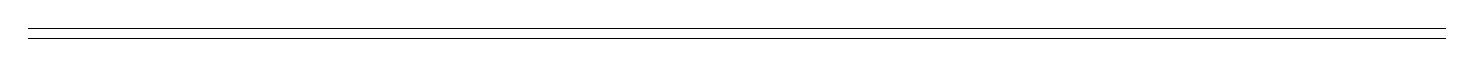
\begin{tikzpicture}
\draw (0,0)--(18,0);
\draw (0,-0.125)--(18,-0.125);
\end{tikzpicture} \\ \\
\textbf{NEXT} more constraint problems.  Maybe in two dimensions. \\ \\
There are lots of good textbook discussions of Lagrange interpolation, the example I had in mind was the Prime Number Theorem, where the common-sense interolation seems to fail.\footnote{We could be in the other situation, where everybody is in the field and three's no theory.}  \\ \\
I wonder if it's possible to write a function which is positive in some parts and negative in the other.  Here's a picture.  It's actually really hard to write a good pattern without going up to $4 \times 4$.   \\ \\
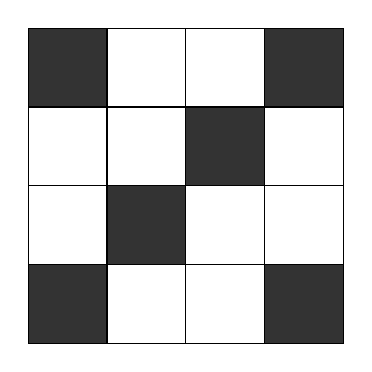
\begin{tikzpicture}



\begin{scope}[xshift=5cm]
\sq{0}{0}{fill=black!80!white};
\sq{1}{0}{};
\sq{2}{0}{};
\sq{3}{0}{fill=black!80!white};
\sq{0}{1}{};
\sq{1}{1}{fill=black!80!white};
\sq{2}{1}{};
\sq{3}{1}{};
\sq{0}{2}{};
\sq{1}{2}{};
\sq{2}{2}{fill=black!80!white};
\sq{3}{2}{};
\sq{0}{3}{fill=black!80!white};
\sq{1}{3}{};
\sq{2}{3}{};
\sq{3}{3}{fill=black!80!white};
\end{scope}


\end{tikzpicture} \\
Can we define a function which is positive on the black square and negative on the white squares? \textbf{Yes} we have to be more specific:
\begin{itemize}
\item monomials $\{ x^m \, y^n : m, n \in \mathbb{N} \}$
\item trig functions $\{ \sin m x \, \sin n y : m, n \in \mathbb{Z}  \}$ 
\end{itemize}  
The second one is more likely, but we can find algebraic curves whose level sets have exactly the contraints we specify (at a cost). \\ \\
My knowledge of 2D interpolation is slim to none and I have to ask around.  So even though PNT\footnote{Prime Number Theorem} is much more difficult, we might proceed first there. \\ \\
Lastly of my outline of examples: \textbf{find a circle that passes through three points}.  Thanks to Decartes, we know a circle has equation like this:
$$ (x - h)^2 + (y- k)^2 = r^2$$
However we may never exactly know what the triples $(h,k,r)$ could be.  In my work, I have to do transformations on the circles, and for each transformation I make, I keep losing accuracy.  Settle for:
$$ (x^2 + y^2) + a\,x + b\,y + c = 0 $$
There are three equations (and three unknowns) so if I add a 4th point, this system will be overdetermined:
$$ \left|
\begin{array}{cllc}
x^2 + y^2 & x & y & 1 \\ \\
x_1^2 + y_1^2 & x_1 & y_1 & 1 \\ \\
x_2^2 + y_2^2 & x_2 & y_2 & 1 \\ \\
x_3^2 + y_3^2 & x_3 & y_3 & 1 \end{array} \right| = 0 $$
It is possible to determine the circle this way.  Let's pick three points: $(0,0),(1,0),(1,1)$ and find the center and radius:
$$ 0 = \left|
\begin{array}{cllc}
x^2 + y^2 & x & y & 1 \\ 
0^2 + 0^2 & 0 & 0 & 1 \\ 
1^2 + 0^2 & 1 & 0 & 1 \\ 
1^2 + 1^2 & 1 & 1 & 1 \end{array} \right| =
\left|
\begin{array}{cll}
x^2 + y^2 & x & y  \\ 
1^2 + 0^2 & 1 & 0  \\ 
1^2 + 1^2 & 1 & 1  \end{array} \right| =
\left|
\begin{array}{cll}
x^2 + y^2 & x & y  \\ 
1 & 1 & 0  \\ 
1 & 0 & 1  \end{array} \right| =
 =(x^2 + y^2) \times 1 - x \times 1  - y \times 1$$
The equation is $x^2 - x + y^2 - y= (x - \frac{1}{2})^2 + (y - \frac{1}{2})^2 - \frac{1}{2}= 0$ so the center is $(x,y,) = (\frac{1}{2},\frac{1}{2})$ and the radius is $r = \frac{1}{\sqrt{2}}$. \\ \\
More difficult is to observe if we map this circle under an \textbf{inversion} the image is still a circle, whose center and radius is less clear:
$$ z \mapsto  - \frac{1}{\overline{z}} \text{ or } (x,y) \mapsto
 \left( \frac{-x}{x^2 + y^2 }, \frac{y}{x^2 + y^2 } \right)  $$
 some proofs are more convincing than others.  Our goal would be to find the radius and center more efficiently. \\ \\
 In the modern day, since we have computers, we might try to \textbf{learn} the center and radius by trial and error.  And we can see how to do that.

\newpage  

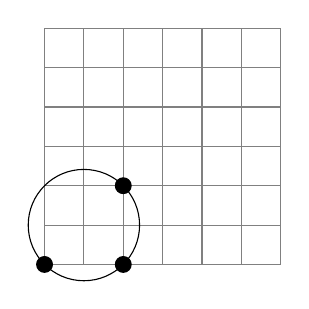
\begin{tikzpicture}

\foreach \a in {0,0.5,...,3}{
\draw[color=black!50!white] (0,\a)--(3,\a);
\draw[color=black!50!white] (\a,0)--(\a,3);
}


\draw[fill=black] (0,0) circle (0.1);
\draw[fill=black] (1,0) circle (0.1);
\draw[fill=black] (1,1) circle (0.1);

\draw[] (0.5,0.5) circle (0.707);

\end{tikzpicture} \\ 
To solve the inversion problem very efficiently: we can use the ``cross product".  This \textit{used} to be taught in older geometry textbooks.  I found the older discussions are more interesting.  Here's a book one way from Morley \& Morley's textbook \textbf{Inversive Geometry} from 1933. \\ \\
$$  \frac{(x_1 - x_2)(x_3 - x_4)}{(x_1 - x_3)(x_2 - x_4)} = 
\frac{\big( f(x_1) - f(x_2) \big) \big( f(x_3) - f(x_4) \big) }{
\big( f(x_1) - f(x_3) \big) \big( f(x_2) - f(x_4) \big) }
 $$
After playing with formulas many many times (a process of centuries) geometers realized this number is preserved under hyperbolic transformations.  One case is obvious $f: x \mapsto x+1$
$$  \frac{( x_1 - x_2)(x_3 - x_4)}{(x_1 - x_3)(x_2 - x_4)} = 
 \frac{ \Big(  (x_1 + 1) - (x_2 + 1)\Big) \Big( (x_3 + 1) - (x_4 + 1) \Big) }{  \Big(  (x_1 + 1) - (x_3 + 1)\Big) \Big( (x_2 + 1) - (x_4 + 1) \Big)  } = \frac{( x_1 - x_2)(x_3 - x_4)}{(x_1 - x_3)(x_2 - x_4)} = 
 $$
Absolutely nothing has happened.  On the other hand if we do the inversion: $g: x \mapsto - \frac{1}{x}$
$$  \frac{( x_1 - x_2)(x_3 - x_4)}{(x_1 - x_3)(x_2 - x_4)} = 
 \frac
{ \Big(  - \frac{1}{x_1} + \frac{1}{x_2} \Big)\Big(  - \frac{1}{x_3} + \frac{1}{x_4} \Big)  } { \Big(  - \frac{1}{x_1} + \frac{1}{x_3} \Big)\Big(  - \frac{1}{x_2} + \frac{1}{x_4} \Big)  }
=  
 \frac
{   \frac{x_1 - x_2}{x_1 x_2} \;\;\; \frac{x_3 - x_4}{x_3 x_4}  }
{   \frac{x_1 - x_3}{x_2 x_4} \;\;\; \frac{x_2 - x_4}{x_2 x_4} }
= 
 \frac{( x_1 - x_2)(x_3 - x_4)}{(x_1 - x_3)(x_2 - x_4)}$$
We need formulas like this because if I run inversion my computer directly, the spacing between the dots on the circle grow more and more uneven.  We can even compute how uneven the circles are getting using some calculus $f(z_0+dz) = f(z_0) + f'(z_0) \, dz$ with $f(z) = - \frac{1}{z}$. \\ 
\includegraphics[width=4in]{inversion-01.png} \\
Notice how I started with a perfect circle and turned it into a straight line. 

\newpage

\noindent Around the year 2000 a group of people figured out a lot about circle inversions (stuff going back to Rene Descarts in the 1600's) but when I ran it on my own computer, the images turned out very bad.  I'll try to reproduce the bad one\dots 

\begin{thebibliography}{}

\item R.L. Graham, J.C. Lagarias, C.L. Mallows, A.R. Wilks, C.H. Yan \\
 \textbf{Apollonian Circle Packings: Number Theory} \texttt{arXiv:math/0009113}
 
\item R.L. Graham, J.C. Lagarias, C.L. Mallows, A.R. Wilks, C.H. Yan \\
\textbf{Apollonian Circle Packings: Geometry and Group Theory I. The Apollonian Group}
 \texttt{arXiv:math/0010298} 

\item R.L. Graham, J.C. Lagarias, C.L. Mallows, A.R. Wilks, C.H. Yan \\
\textbf{Apollonian Circle Packings: Geometry and Group Theory II. Super-Apollonian Group and Integral Packings}
\texttt{arXiv:math/0010302}


\item R.L. Graham, J.C. Lagarias, C.L. Mallows, A.R. Wilks, C.H. Yan \\
\textbf{Apollonian Circle Packings: Geometry and Group Theory III. Higher Dimensions}
\texttt{arXiv:math/0010324} 

\item \texttt{arXiv:math/0101066} 
\textbf{Beyond the Descartes circle theorem}
Jeffrey C. Lagarias, Colin L. Mallows, Allan R. Wilks

\end{thebibliography}

\includegraphics[width=5in]{inversion-02.png} \\ 
(from Wikipedia)

\end{document}